\section{Aylanma harakatni uzatish}

\begin{enumerate}

\item Harakat I g'ildirakdan tasmali uzatma yordamida uzatiladi. Agar I g'ildirak minutiga 2400 marta aylansa, g'ildiraklarning radiuslari esa mos ravishda 3 va 6 sm bo'lsa, ikkinchi g'ildirakning burchak tezligi qanday (rad/s) bo'ladi?
\begin{enumerate}[label=\Alph*)]
\item $2\pi$
\item $40\pi$
\item $20\pi$
\item $10\pi$
\end{enumerate}

\item Zanjirli uzatma yordamida bog'langan ikkita tishli g'ildirakning biridagi tishlar soni $N_1$ ikkinchisidagi tishlar soni $N_2$ dan 4 marta ko'p bo'lsa, g'ildiraklarning burchak tezliklari orasidagi munosabat qanday bo'ladi?
\begin{enumerate}[label=\Alph*)]
\item $\omega_2 = 2\omega_1$
\item $\omega_2 = 4\omega_1$
\item $\omega_1 = 2\omega_2$
\item $\omega_1 = 4\omega_2$
\end{enumerate}

\item Tasma orqali biriktirilgan ikki shkivning radiuslari 10 sm va 15 sm. Birinchi shkivning chiziqli tezligi 2 m/s bo'lsa, ikkinchi shkivning chiziqli tezligini toping (m/s)?
\begin{enumerate}[label=\Alph*)]
\item 1,3
\item 2
\item 3
\item 4,3
\end{enumerate}

\item Tishlarining soni $N_1 = 150$ va $N_2$ bo'lgan shesternalar bir-biriga bog'langan. Birinchi shesterna har sekundda 20 marta aylanganda, ikkinchisi har minutda 250 marta aylansa $N_2$ - ?
\begin{enumerate}[label=\Alph*)]
\item 720
\item 250
\item 150
\item 750
\end{enumerate}

\item "Penza" velosipedi g'ildiragining diametri 70 sm, yetakchi tishli g'ildiragining tishlari 48 ta, yetaklanuvchi tishli g'ildiragining tishlari 18 ta. Pedallarning aylanish chastotasi 1 ayl/s bo'lsa, velosipedchi qanday tezlik bilan harakatlanmoqda (m/s)?
\begin{enumerate}[label=\Alph*)]
\item 3,7
\item 4,3
\item 6,6
\item 5,9
\end{enumerate}

\item Yig'ma "Kama" velosipedi g'ildiragining diametri 50 sm, tishli g'ildiragining tishlari 48 ta va 15 ta hamda pedallarning aylanish chastotasi 1 ayl/s bo'lsa, undagi velosipedchi qanday tezlik bilan harakatlanadi (m/s)?
\begin{enumerate}[label=\Alph*)]
\item 20
\item 10
\item 5
\item 0,2
\end{enumerate}

\item Tasma orqali biriktirilgan ikki shkivning radiuslari 10 sm va 15 sm. Birinchi shkivning burchak tezligi 2 rad/s bo'lsa, ikkinchi shkivning burchak tezligini toping (rad/s).
\begin{enumerate}[label=\Alph*)]
\item 1,3
\item 2
\item 3
\item 4,3
\end{enumerate}

\item Gidroturbina ishchi g'ildiragining radiusi bug' turbinasinikiga qaraganda 8 marta katta, aylanish chastotasi esa 40 marta kichik. Turbina g'ildiraklari to'g'inidagi nuqtalarining tezliklarini taqqoslang.
\begin{enumerate}[label=\Alph*)]
\item 1:4
\item 1:5
\item 1:2
\item 2:5
\end{enumerate}

\item Radiusi 32 sm bo'lgan katta shkiv 180 ayl/min chastota bilan aylanmoqda va u radiusi 24 sm bo'lgan kichkina shkiv bilan tasma orqali bog'langan. Kichik shkivning burchak tezligini (rad/s) toping.
\begin{enumerate}[label=\Alph*)]
\item 11/3
\item $8\pi$
\item $3\pi$
\item $6\pi$
\end{enumerate}

\item Rasmda traktorning katta g'ildiragidagi A nuqtaning yerga nisbatan oniy tezligi $4\sqrt{2}$ m/s bo'lsa, B nuqtaning yerga nisbatan oniy tezligini (m/s) toping.

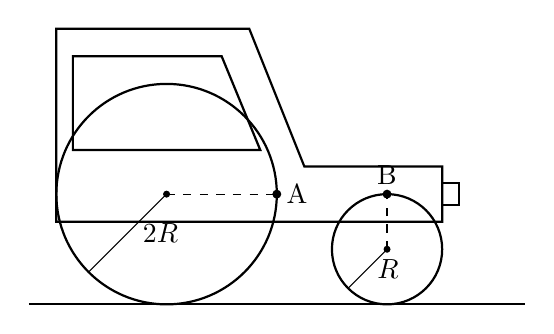
\begin{tikzpicture}[>=stealth, scale=0.7]
    % Yer chizig'i
    \draw[thick] (0,0) -- (9,0);

    % Katta g'ildirak (Orqa)
    \draw[thick] (2.5,2) circle (2);
    \filldraw (2.5,2) circle (1.5pt); % Markaz
    \draw[dashed] (2.5,2) -- (4.5,2); % Gorizontal nuqtali chiziq
    \filldraw (4.5,2) circle (2pt) node[right] {A}; % A nuqta
    \draw (2.5,2) -- ++(225:2) node[midway, right, xshift=2pt] {$2R$}; % Radius 2R

    % Kichik g'ildirak (Oldi)
    \draw[thick] (6.5,1) circle (1);
    \filldraw (6.5,1) circle (1.5pt); % Markaz
    \draw[dashed] (6.5,1) -- (6.5,2); % Vertikal nuqtali chiziq
    \filldraw (6.5,2) circle (2pt) node[above] {B}; % B nuqta
    \draw (6.5,1) -- ++(225:1) node[midway, right] {$R$}; % Radius R

    % Traktor tanasi (Outline)
    \draw[thick] (0.5,1.5) -- (0.5,5) -- (4,5) -- (5,2.5) -- (7.5,2.5) -- (7.5,1.5) -- cycle;
    
    % Oyna/Kabina detali
    \draw[thick] (0.8,2.8) -- (4.2,2.8) -- (3.5,4.5) -- (0.8,4.5) -- cycle;
    
    % Old chiroq/detal
    \draw[thick] (7.5, 2.2) -- (7.8, 2.2) -- (7.8, 1.8) -- (7.5, 1.8);

\end{tikzpicture}

\begin{enumerate}[label=\Alph*)]
\item 12
\item 10
\item 8
\item 24
\end{enumerate}

\item Bitta o'qqa mahkamlangan ikki shkivning radiuslari mos ravishda 20 sm va 25 sm. Ikkinchi shkivning aylanish davri 4 s bo'lsa, birinchi shkivning aylanish chastotasini toping (1/s).
\begin{enumerate}[label=\Alph*)]
\item 4
\item 0,25
\item 5
\item 0,2
\end{enumerate}

\item Bir nuqtaga mahkamlangan radiuslari 10 sm va 25 sm bo'lgan shkivlardan birinchisining aylanish davri 10 s bo'lsa, ikkinchisining aylanish davrini toping (s).
\begin{enumerate}[label=\Alph*)]
\item 15
\item 4
\item 25
\item 10
\end{enumerate}

\item Bitta o'qqa mahkamlangan radiuslari 15 sm va 25 sm bo'lgan shkivlardan kichigining eng chekka nuqtalaridagi chiziqli tezligi 2,25 m/s. Katta shkivning eng chekka nuqtalaridagi chiziqli tezligini toping (m/s).
\begin{enumerate}[label=\Alph*)]
\item 6,25
\item 2,5
\item 1,5
\item 3,75
\end{enumerate}

\item Bitta o'qqa mahkamlangan radiuslari 20 sm va 35 sm bo'lgan shkivlardan kattasining eng chekka nuqtalaridagi markazga intilma tezlanishi 1,4 $m/s^2$. Kichik shkiv eng chekka nuqtalarining markazga intilma tezlanishini toping ($m/s^2$).
\begin{enumerate}[label=\Alph*)]
\item 25
\item 3,5
\item 2
\item 0,8
\end{enumerate}

\item Bitta o'qqa mahkamlangan radiuslari 15 sm va 25 sm bo'lgan shkivlardan kichigining eng chekka nuqtalarining aylanish davri 2,25 s. Katta shkivning eng chekka nuqtalarining aylanish davrini toping (s).
\begin{enumerate}[label=\Alph*)]
\item 6,25
\item 2,5
\item 1,5
\item 2,25
\end{enumerate}

\item Disk o'q atrofida o'zgarmas tezlik bilan aylanmoqda. Aylanish o'qidan har xil masofada joylashgan 1, 2 va 3-nuqtalarning markazga intilma tezlanishlari qanday munosabatda bo'ladi?

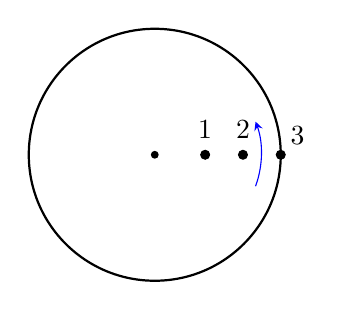
\begin{tikzpicture}[>=stealth, scale=0.8]
    % Diskning asosi (aylana)
    \draw[thick] (0,0) circle (2);
    
    % Aylanish o'qi (markazdagi nuqta)
    \filldraw (0,0) circle (1.5pt);
    
    % Nuqtalar (1, 2 va 3) bitta radius bo'ylab joylashgan
    % 1-nuqta (markazga yaqin)
    \filldraw (0.8,0) circle (2pt);
    \node[above] at (0.8,0.1) {1};
    
    % 2-nuqta (o'rtada)
    \filldraw (1.4,0) circle (2pt);
    \node[above] at (1.4,0.1) {2};
    
    % 3-nuqta (disk chetida)
    \filldraw (2,0) circle (2pt);
    \node[above right] at (2,0) {3};
    
    % Ixtiyoriy: Aylanish yo'nalishini ko'rsatuvchi yoy
    \draw[->, blue] (1.6, -0.5) arc (-20:20:1.5);

\end{tikzpicture}

\begin{enumerate}[label=\Alph*)]
\item $a_1 > a_2 > a_3$
\item $a_1 = a_2 = a_3$
\item $a_1 = a_2 > a_3$
\item $a_1 < a_2 < a_3$
\end{enumerate}

\end{enumerate}


\begin{table}[h!]
\centering
\caption{10-§. Aylana bo'ylab tekis harakatni uzatish bo'yicha to'g'ri javoblar jadvali}
\begin{tabular}{|l|c|c|c|c|c|c|c|c|c|c|}
\hline
\textbf{Savol №} & 1 & 2 & 3 & 4 & 5 & 6 & 7 & 8 & 9 & 10 \\ \hline
\textbf{Javob}   & B & D & B & A & D & C & A & B & B & C \\ \hline
\hline
\textbf{Savol №} & 11 & 12 & 13 & 14 & 15 & 16 &  & & & \\ \hline
\textbf{Javob}   & B & D & E & D & D & D &  & & & \\ \hline
\end{tabular}
\end{table}

